\documentclass[lettersize,journal]{IEEEtran}
\usepackage{amsmath,amsfonts}
\usepackage{algorithmic}
\usepackage{algorithm}
\usepackage{array}
\usepackage[caption=false,font=normalsize,labelfont=sf,textfont=sf]{subfig}
\usepackage{textcomp}
\usepackage{stfloats}
\usepackage{url}
\usepackage{verbatim}
\usepackage{graphicx}
\usepackage{xcolor}
\usepackage{csquotes}
\usepackage{makecell}
% my added packages and commands =======================
\usepackage[numbers]{natbib} %removed cite package

\usepackage{tikz}
\usetikzlibrary{positioning,shapes.geometric}
\usepackage{adjustbox}
\usepackage{listings}
\usepackage{caption}         

\newcommand{\highlight}[1]{\textcolor[RGB]{00,100,100}{#1}}
\newcommand{\todo}[1]{\textcolor{red}{#1}}

\captionsetup[lstlisting]{justification=centering, singlelinecheck=false}
\providecommand{\gls}[1]{#1}
\definecolor{rank1}{HTML}{70FF70}
\definecolor{rank2}{HTML}{858585}
\definecolor{rank3}{HTML}{454545}
\definecolor{rank4}{HTML}{000000}
\newcommand{\SIMSESpec}{\texttt{SIMSE\_Spec}}
\newcommand{\LoneSpec}{\texttt{L1\_Spec}}
\newcommand{\JTFS}{\texttt{JTFS}}
\newcommand{\DTWEnv}{\texttt{DTW\_Envelope}}
\newcommand{\LossSelect}{\textbf{Loss Selection}}
\newcommand{\SynthSelect}{\textbf{Synthesis Selection}}
\newcommand{\PeriodicLoss}{\textbf{Periodic Loss}}
\newcommand{\OutDomain}{\textbf{Out-Domain Generation}}
\newcommand{\BPNoise}{\textbf{BP-Noise}}  
\newcommand{\AddSineSaw}{\textbf{Add-SineSaw}}  
\newcommand{\AmpMod}{\textbf{Noise-AM}}  
\newcommand{\FMMod}{\textbf{SineSaw-AM}}  

% code_style.tex
\usepackage{xcolor}
\usepackage{tikz}

\newcommand{\greencircle}{%
    
\begin{tikzpicture}
        \fill[green] (0,0) circle (4pt); % Adjust the size here if needed
    \end{tikzpicture}%
}

\newcommand{\greenstar}{%
    
\begin{tikzpicture}[scale=0.22]
        \fill[green] 
            (0,1) 
            -- (0.2245,0.309) 
            -- (1,0.309) 
            -- (0.3633,-0.118) 
            -- (0.5878,-0.809) 
            -- (0,-0.382) 
            -- (-0.5878,-0.809) 
            -- (-0.3633,-0.118) 
            -- (-1,0.309) 
            -- (-0.2245,0.309) 
            -- cycle;
    \end{tikzpicture}%
}

\newcommand{\redcircles}{
    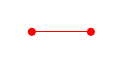
\begin{tikzpicture}[scale=0.75, line cap=round, line join=round]
        % Define coordinates for circles
        \coordinate (A) at (0,0);
        \coordinate (B) at (1,0);
        \coordinate (C) at (2,0);
        \coordinate (D) at (3,0);
        
        % Draw circles
        \foreach \point in {A,B} 
            \fill[red] (\point) circle (2pt);
        
        % Connect circles with lines
        \draw[red] (A) -- (B);
    \end{tikzpicture}%
}

\lstdefinelanguage{Faust}{
    morekeywords={import, process, environment, declare, with, if, else, while, for, int, float, true, false},
    sensitive=true,
    morecomment=[l]{//}, % Line comment
    morecomment=[s]{/*}{*/}, % Block comment
    morestring=[b]", % Strings
}

% Customize the appearance of the code
\lstset{
    language=Faust,
    backgroundcolor=\color{lightgray!20},
    basicstyle=\ttfamily\small,
    keywordstyle=\color{blue}\bfseries,
    stringstyle=\color{orange},
    commentstyle=\color{green}\itshape,
    showstringspaces=false,
    numbers=left,
    numberstyle=\tiny,
    frame=single,
    breaklines=true
}

% Suppress the "Listing #" label and caption text
% \captionsetup[lstlisting]{
%     labelformat=empty,
%     labelsep=none,
%     font=normalfont,
%     skip=0pt
% }


%  ================================
\begin{document}
\bibliographystyle{IEEEtran}


\title{Evaluating Sound Similarity Metrics for Differentiable, Iterative Sound-Matching}

\author{Amir Salimi, Abram Hindle, Osmar R. Za{\"i}ane}
\maketitle
 
\begin{IEEEkeywords}
Audio synthesis, differentiable digital signal processing, music information retrieval, sound-matching
\end{IEEEkeywords}
\hphantom{\vphantom{\begin{minipage}{\textwidth}\bibliography{references}\end{minipage}}}


\section{Background and Past Works}
\label{sec:background}
This section provides an introduction to digital audio synthesis, audio similarity measures, and a formal definition of sound-matching. We then provide a typology of sound-matching tasks using previous works as well as conceptual approaches that may be promising but though underexplored. Finally, a discussion on the current gaps of knowledge in the field is provided.


\subsection{Digital Audio Synthesis}
\label{sec:diffSynth}
A digital audio synthesizer is any software used for the creation and manipulation of digital audio. Digital synthesizers use signal processing chains with a variety of digital signal processing (\gls{DSP}) functions to create sounds. These functions are often parametric, and the set of parameters given to the synthesizer's chain of DSP functions is called a synthesizer program.

The simplest form of DSP function is a sinusoidal tone. For example, consider:
\[ x(n) = sin( 2\pi n T)\]

where $T$ represents time in seconds, and $n$ is the frequency parameter. If $n$ is 1, then $x(n)$ would be a waveform with a frequency of 1 hertz, meaning that the value of $x(n)$ oscillates to the same point once every second. Waveform generators are called oscillators for this reason. 

Since the advent of digital signal processing in the 1960s~\cite{stranneby2004digital}, a wide variety of parametric audio generation functions have been proposed~\cite{lyons1997understanding,russ1999sound,shier2020spiegelib}. This includes oscillators, filters, equalizers, and envelopes, which can be used sequentially or in parallel~\cite{lyons1997understanding,russ1999sound}. Sound design with a synthesizer is done by modifying the parameters of the functions until reaching a desired output~\cite{roads1996computer,pinch2004analog}.

Particularly in earlier works, frequency/amplitude modulators (\gls{FM}/\gls{AM}) has been the synthesizer of choice in sound-matching~\cite{horner1993machine,mitchell2007evolutionary,vahidi2023mesostructures}. This synthesis method is simple to implement, yet very expressive~\cite{chowning1973synthesis}. One of the earliest foundational sound-matching works is the analytical approach by Justice~\cite{justice1979analytic} toward the decomposition and recreation of sounds with FM synthesis using one carrier, one modulator, and the corresponding envelopes:
\[ f(t) = I_c(t) \cos(\omega_c t + I_m(t) \cos(\omega_m t))
\]
Where $f(t)$ is the output signal, $I_c(t)$ is the carrier amplitude, $\omega_c$ is the carrier frequency, and $I_m(t)$ and $\omega_m$ are the envelope and frequency for the modulator~\cite{justice1979analytic}. 

Compared to the number of possible approaches to sound synthesis, a relatively small subset of synthesis methods have been analyzed in \textit{isolation} for sound-matching. Notable methods here are additive and/or subtractive synthesizers~\cite{engel2020ddsp,masuda2023improving,salimi2020make} and physical modeling~\cite{riionheimo2003parameter,han2024learning}.

\highlight{
What we mean here by \textit{isolation} is that the effect of the synthesizer's parameters (how they change the output sound and experiment outcome) is easily tractable. Recent computational advancements have allowed the use of complex Virtual Studio Technology (VST)\cite{steinberg1996vst} synthesizers in sound-matching~\cite{yee2018automatic,esling2019flow}, however, this has the trade-off here is the obfuscation of the interactions between the synthesizer functions, the loss, and the final outcome, among other distinctions which we will discuss in this section. 
}

An important recent development in digital audio synthesis is the increase of interest in differentiable DSP (\gls{DDSP})~\cite{engel2020ddsp}. DDSP is a general term for applications that combine machine learning techniques such as gradient descent~\cite{goodfellow2016deep,boyd2004convex} with DSP. Implementing complex DSP functions in a differentiable manner can be challenging, and effective differentiable audio similarity measures require careful mathematical expression of the desired attributes of sound. These issues have likely contributed to the limited exploration of this domain~\cite{masuda2021soundmatch,vahidi2023mesostructures,uzrad2024diffmoog}. 

% \subsection{Sound Representation and Loss Functions}
% \label{sec:loss_funcs}
% A digital sound (or an audio signal) is a series of numbers~\cite{smith1991viewpoints,smith2007mathematics}. To compare two digital sounds, the two corresponding series are passed to a function that measures their similarity. Two signals can sound identical to our ears, without having any values in common~\cite{moore2012introduction}. This necessitates the use of proxy representations (or feature extractors) when comparing sounds automatically. Similarity between the target sound and the synthesizer output is then measured by some form of subtraction and summation of the proxy representations.

% In sound-matching, particularly in a Deep Learning (\gls{DL}) context~\cite{goodfellow2016deep}, the similarity function can also be called a \textit{loss} function, where the emphasis is on measurement and reduction of the distance between target and output. It is important to note that there is a close relationship between the loss function $L$ and the sound representation function $\phi$. $L$ is the result of a distance measure $d$ applied to the features extracted by $\phi$. 

% \[
% L(\theta, t) = d\langle\phi(t),\phi(x)\rangle
% \]

% \noindent

% A proxy representation is the output of the function \( \phi \), which can be thought of as a feature extraction function that maps the sounds \( t \) and \( x \) to their respective representations. 
% The proportionality or distance metric $d$ has typically been the L1 distance~\cite{turian2020sorry,richard2025model}, calculated as the mean of the absolute difference between every point in the proxy representation~\cite{engel2020ddsp,vahidi2023mesostructures}:
% \[
% L(\theta, t) = \left\| \phi(t) - \phi(x) \right\|_1
% \]

% Here we discuss four methods of audio representation and the corresponding loss functions. Three of which have been used in previous works, and a novel method not previously used in iterative sound-matching. 

% \subsubsection{Parameter Loss}
% A common measure of similarity in sound-matching is the distance between synthesizer parameter sets, referred to as ``P-Loss"~\cite{han2023perceptual}. Typically, for the implementation of P-Loss the parameter sets are treated as vectors in space, and L1 or L2 distance is applied. There are two major limitations to this approach: First, the target and output sound must be made by the same synthesizer; otherwise the parameter sets cannot be compared (see Section~\ref{sec:matching_types}). Second, the relationship between synthesizer parameters and the audio output is not linear~\cite{shier2020spiegelib,han2023perceptual,esling2019flow}. 

% \subsubsection{Fourier Spectrograms}
% \label{sec:fourier_specs}
% Fourier-based transformations such as short-time Fourier transforms (\gls{STFT}), Mel-spectrograms, and Mel-frequency cepstral coefficients have been viewed as the de facto and state-of-the-art representation of audio~\cite{beauchamp2003error,mitchell2007evolutionary,yee2018automatic}, however, there are many issues associated with their use in sound-matching~\cite{turian2020sorry,vahidi2023mesostructures,han2023perceptual,uzrad2024diffmoog}. Fourier transformations allow for the conversion of a signal from the time-domain to the frequency domain. Audio spectrograms can be generated by segmentation of a piece of audio into overlapping windows followed by the application of Fourier transforms to each window. They are costly to compute, but provide a better temporal view of changes in frequency content~\cite{muller2007dynamic,smith2007mathematics}. There are different types of spectrograms that have a basis in Fourier transformations, but the most notable and commonly used is the STFT.  

% What we call \textit{Fourier-based Spectrograms} are variations on the STFT approach. For example, Mel-Spectrograms \textit{bin} frequencies on a near-logarithmic scale to better match human perception of frequencies~\cite{muller2007dynamic}. Multi-scale spectrograms (\gls{MSS}) used in recent works are a simple weighted average of multiple spectrograms with different parameters such as window size, number of frequency bins, and hop size~\cite{engel2020ddsp,vahidi2023mesostructures}; this may provide some improvements at a higher computational cost~\cite{turian2020sorry,engel2020ddsp}.


% \subsubsection{Joint-Time Frequency Spectrum}
% Recent works have focused on the limitations of parameter and spectral loss functions in sound-matching~\cite{vahidi2023mesostructures,uzrad2024diffmoog}, seeking to create more effective general solutions for the comparison of audio. 
% Noting the aforementioned weaknesses of comparing STFT spectrograms, Vahidi \textit{et al.} proposed differentiable Joint-Time Frequency Scattering (\gls{JTFS})~\cite{anden2015joint} as an alternative to spectrogram loss in sound-matching, and showed improved performance in sound-matching with differentiable chirplet synthesizers~\cite{vahidi2023mesostructures}. JTFS is the result of the application of a 2D wavelet transformation to the time-frequency representation of a signal~\cite{anden2015joint}. 

% \subsubsection{Dynamic Envelope Warping}
% Dynamic Time Warping (DTW) is a method for measuring similarity between multi-dimensional time-series~\cite{rabiner1993fundamentals,muller2007dynamic,giorgino2009computing}. Given any two time-series $X = \{x_1,x_2,...,x_m\}$ and $Y = \{y_1,y_2,...,y_n\}$, we have indices $i\in\{1...m\}$ and $j\in\{1...n\}$ defining $X$ and $Y$. When the series are \textit{warped}, these indices change to expand or contract different portions of the series. To borrow the notation given by Muller~\cite{muller2007dynamic}, warped indices are a sequence $p=(p_1,...,p_L)$, where \(p_\ell = (m_\ell, n_\ell) \in [1 : m] \times [1 : n] \text{ for } \ell \in [1 : L]\), meaning that the indices for $X$ and $Y$ are reorganized under special conditions. In classical DTW, these conditions are \textit{monotonicity}, \textit{boundary matching}, and \textit{single step-size}.

% DTW measures the distance between the time-series \textit{after} alignments, typically using Euclidean distance. The distance between a time-series and shifted versions of itself would be 0, regardless of shift amount~\cite{tavenard.blog.dtw}. Additional rules can be imposed to keep alignments locally constrained~\cite{itakura1975minimum,sakoe1978dynamic}.

% \subsection{Automatic Sound Matching}
% \label{sec:sound_matching_definition}
% Sound-matching requires a number of modular parts: the choice of synthesizer $g$, the target sounds of interest, the representation function $\phi$, and the heuristic for finding the optimal $\theta$. To give a formal definition of sound-matching, we expand the definition given by recent works~\cite{vahidi2023mesostructures,han2023perceptual}. The major components are as follows: 
% \begin{itemize}
%     \item $g(\theta)$: Parametric audio synthesizer $g$ which takes on parameters $\theta$ 
%     \item $x$: The output of $g$, given a set of parameters $\theta$ or $g(\theta) = x$ 
%     \item $t$: The target sound which we want to replicate or imitate. 
%     \item $\phi$: Representation function or feature extractor. $\phi$ is applied to $x$ and $t$ to facilitate their comparison by the loss function.
%     \item $L$: Loss or error function. $L(\theta,t)$ is a measure of distance between $x$ and $t$. Often proportional to the subtraction of their representations, or $ \phi(x) - \phi(t)$
% \end{itemize}

% \highlight{It could be argued that the implementation of these components is not an optimization problem with a correct answer, but a \textit{creative} endeavor depending on the artist's needs}. Consider the hypothetical case where two sound-designers are searching for an 8-bit~\cite{collins2007loop} version of a high quality, organic snare drum: in such a case, there is no optimal solution, and the space of possible answers is extremely large. Here, it is possible (if not highly likely) that the two artists would select different samples given a number of possible samples to choose from. 

% \subsection{Past Works}
% Given that sound-matching is ultimately an imitation of a creative endeavor, it might be no surprise that it can be categorized into different subtypes. 


\subsection{Sound Representation and Loss Functions}
\label{sec:loss_funcs}
A digital sound (or an audio signal) is a series of numbers~\cite{smith1991viewpoints,smith2007mathematics}. To compare two digital sounds, the two corresponding series are passed to a function that measures their similarity. Two signals can sound identical to our ears, without having any values in common~\cite{moore2012introduction}. This necessitates the use of proxy representations (or feature extractors) when comparing sounds automatically. Similarity between the target sound and the synthesizer output is then measured by some form of subtraction and summation of the proxy representations.

In sound-matching, particularly in a Deep Learning (\gls{DL}) context~\cite{goodfellow2016deep}, the similarity function can also be called a \textit{loss} function, where the emphasis is on measurement and reduction of the distance between target and output. It is important to note that there is a close relationship between the loss function $L$ and the sound representation function $\phi$. $L$ is the result of a distance measure $d$ applied to the features extracted by $\phi$. 

\[
L(\theta, t) = d\langle\phi(t),\phi(x)\rangle
\]

\noindent

A proxy representation is the output of the function \( \phi \), which can be thought of as a feature extraction function that maps the sounds \( t \) and \( x \) to their respective representations. 
The proportionality or distance metric $d$ has typically been the L1 distance~\cite{turian2020sorry,richard2025model}, calculated as the mean of the absolute difference between every point in the proxy representation~\cite{engel2020ddsp,vahidi2023mesostructures}:
\[
L(\theta, t) = \left\| \phi(t) - \phi(x) \right\|_1
\]

Here we discuss four methods of audio representation and the corresponding loss functions. Three of which have been used in previous works, and a novel method not previously used in iterative sound-matching. 

\subsubsection{Parameter Loss}
A common measure of similarity in sound-matching is the distance between synthesizer parameter sets, referred to as ``P-Loss"~\cite{han2023perceptual}. Typically, for the implementation of P-Loss the parameter sets are treated as vectors in space, and L1 or L2 distance is applied. There are two major limitations to this approach: First, the target and output sound must be made by the same synthesizer; otherwise the parameter sets cannot be compared (see Section~\ref{sec:matching_types}). Second, the relationship between synthesizer parameters and the audio output is not linear~\cite{shier2020spiegelib,han2023perceptual,esling2019flow}. 

\subsubsection{Fourier Spectrograms}
\label{sec:fourier_specs}
Fourier-based transformations such as short-time Fourier transforms (\gls{STFT}), Mel-spectrograms, and Mel-frequency cepstral coefficients have been viewed as the de facto and state-of-the-art representation of audio~\cite{beauchamp2003error,mitchell2007evolutionary,yee2018automatic}, however, there are many issues associated with their use in sound-matching~\cite{turian2020sorry,vahidi2023mesostructures,han2023perceptual,uzrad2024diffmoog}. Fourier transformations allow for the conversion of a signal from the time-domain to the frequency domain. Audio spectrograms can be generated by segmentation of a piece of audio into overlapping windows followed by the application of Fourier transforms to each window. They are costly to compute, but provide a better temporal view of changes in frequency content~\cite{muller2007dynamic,smith2007mathematics}. There are different types of spectrograms that have a basis in Fourier transformations, but the most notable and commonly used is the STFT.  

What we call \textit{Fourier-based Spectrograms} are variations on the STFT approach. For example, Mel-Spectrograms \textit{bin} frequencies on a near-logarithmic scale to better match human perception of frequencies~\cite{muller2007dynamic}. Multi-scale spectrograms (\gls{MSS}) used in recent works are a simple weighted average of multiple spectrograms with different parameters such as window size, number of frequency bins, and hop size~\cite{engel2020ddsp,vahidi2023mesostructures}; this may provide some improvements at a higher computational cost~\cite{turian2020sorry,engel2020ddsp}.


\subsubsection{Joint-Time Frequency Spectrum}
Recent works have focused on the limitations of parameter and spectral loss functions in sound-matching~\cite{vahidi2023mesostructures,uzrad2024diffmoog}, seeking to create more effective general solutions for the comparison of audio. 
Noting the aforementioned weaknesses of comparing STFT spectrograms, Vahidi \textit{et al.} proposed differentiable Joint-Time Frequency Scattering (\gls{JTFS})~\cite{anden2015joint} as an alternative to spectrogram loss in sound-matching, and showed improved performance in sound-matching with differentiable chirplet synthesizers~\cite{vahidi2023mesostructures}. JTFS is the result of the application of a 2D wavelet transformation to the time-frequency representation of a signal~\cite{anden2015joint}. 

\subsubsection{Dynamic Envelope Warping}
Dynamic Time Warping (DTW) is a method for measuring similarity between multi-dimensional time-series~\cite{rabiner1993fundamentals,muller2007dynamic,giorgino2009computing}. Given any two time-series $X = \{x_1,x_2,...,x_m\}$ and $Y = \{y_1,y_2,...,y_n\}$, we have indices $i\in\{1...m\}$ and $j\in\{1...n\}$ defining $X$ and $Y$. When the series are \textit{warped}, these indices change to expand or contract different portions of the series. To borrow the notation given by Muller~\cite{muller2007dynamic}, warped indices are a sequence $p=(p_1,...,p_L)$, where \(p_\ell = (m_\ell, n_\ell) \in [1 : m] \times [1 : n] \text{ for } \ell \in [1 : L]\), meaning that the indices for $X$ and $Y$ are reorganized under special conditions. In classical DTW, these conditions are \textit{monotonicity}, \textit{boundary matching}, and \textit{single step-size}.

DTW measures the distance between the time-series \textit{after} alignments, typically using Euclidean distance. The distance between a time-series and shifted versions of itself would be 0, regardless of shift amount~\cite{tavenard.blog.dtw}. Additional rules can be imposed to keep alignments locally constrained~\cite{itakura1975minimum,sakoe1978dynamic}.
% \textcolor{red}{DTW was originally used for signal comparison but using it the way we do is novel}


\subsection{Automatic Sound Matching}
\label{sec:sound_matching_definition}
The problem of sound-matching has been tackled from a variety of perspectives as it involves a number of modular parts: the choice of synthesizer $g$, the target sounds of interest, the representation function $\phi$, and the heuristic for finding the optimal $\theta$. To give a formal definition of sound-matching, we expand the definition given by recent works~\cite{vahidi2023mesostructures,han2023perceptual}. The major components are as follows: 
\begin{itemize}
    \item $g(\theta)$: Parametric audio synthesizer $g$ which takes on parameters $\theta$ 
    \item $x$: The output of $g$, given a set of parameters $\theta$ or $g(\theta) = x$ 
    \item $t$: The target sound which we want to replicate or imitate. 
    \item $\phi$: Representation function or feature extractor. $\phi$ is applied to $x$ and $t$ to facilitate their comparison by the loss function.
    \item $L$: Loss or error function. $L(\theta,t)$ is a measure of distance between $x$ and $t$. Often proportional to the subtraction of their representations, or $ \phi(x) - \phi(t)$
\end{itemize}

\highlight{It could be argued that the implementation of these components is not an optimization problem with a correct answer, but a \textit{creative} endeavor depending on the artist's needs}. Consider the hypothetical case where the goal might be to create an 8-bit~\cite{collins2007loop} version of a high quality, organic snare drum: in such a case, there is no optimal or ``correct" version of an 8-bit snare sound. 

\subsection{In-Domain versus Out-of-Domain}
\label{sec:in-domain}
The choice of domain depends on whether we want to use the same synthesizer for the target and output sounds, the scenario that is called \textit{in-domain}, or have target sounds that came from sources other than the synthesizer, or \textit{out-of-domain}. To paraphrase the description given by Masuda \textit{et al.}~\cite{masuda2021soundmatch}, if $g$, the synthesizer of choice, can accurately replicate the target sound $t$, or put differently, if $t$ itself is an output of $g$, then the sound-matching task is \textit{in-domain}. If $t$ is not an output of $g$, then the sound-matching task is \textit{out-of-domain}. In-domain tasks in general are simpler, and often there is a guarantee that there is a correct answer to the sound-matching problem, particularly if the goal is accurate replication of the sound. If the target sound is out-of-domain, replication is not guaranteed, and the goal becomes the \textit{imitation} of some aspect of sound. 

Regardless of the domain, the generation goal can be \textit{replication} or \textit{imitation} of the target sound. In replication, the goal is to make an identical copy of the target sound. Imitation is an artistic pursuit and harder to define, since the goal is to make new sounds that only retain a subset of the target's sonic features. While closely related to the in-domain versus out-of-domain problem, the choice of replication versus imitation is more dependent on how the loss and representation functions are defined. 

\subsection{Supervised vs Iterative}
\label{sec:optimization}
% The goal of sound-matching is to find the optimal parameters $\theta^*$ that minimize the loss between the synthesizer output and the target sound. 
% \[
% \theta^* = \arg\min_{\theta} L(\theta,t)
% \]

% The \textit{heuristics} (i.e., how the parameters are approximated) used in past works can be broadly split into two categories:
% \begin{enumerate}
%     \item Direct optimization methods~\cite{horner1993machine,mitchell2007evolutionary,yee2018automatic,vahidi2023mesostructures}. This requires a target example, and a loss function that measures the difference between the target and synthesizer outputs. Given these two necessary pieces, direct optimization refers to the iterative generation of a sound output, measurement the distance between target and output, and applying updates to the parameters. 
    
%     \item Supervised (or inference) methods which use datasets of sound corresponding parameters to learn the generation objective. Often with a large number of input and output examples and use of DNNs~\cite{engel2020ddsp,salimi2020make,yee2018automatic,esling2019flow}. Often, these models output their parameter predictions in a single step (or 1-shot).  
    

% \end{enumerate}



\end{document}


